% This is samplepaper.tex, a sample chapter demonstrating the
% LLNCS macro package for Springer Computer Science proceedings;
% Version 2.21 of 2022/01/12
%
\documentclass[runningheads]{llncs}
%
\usepackage[T1]{fontenc}
% T1 fonts will be used to generate the final print and online PDFs,
% so please use T1 fonts in your manuscript whenever possible.
% Other font encondings may result in incorrect characters.
%
\usepackage{graphicx}
% Used for displaying a sample figure. If possible, figure files should
% be included in EPS format.
%
% If you use the hyperref package, please uncomment the following two lines
% to display URLs in blue roman font according to Springer's eBook style:
\usepackage{hyperref}
\usepackage{color}
\renewcommand\UrlFont{\color{blue}\rmfamily}
%%%%%%%%%%%%%%%%%%%%%%%%%%%%%%%%%%%%%%%%%%%%%%%%%%%%%%%%%%%%%%%%%%%%%%%%%%%%%%%%
% Custom packages:
\usepackage[inline]{enumitem}
\usepackage[noend]{algpseudocode}
\usepackage[super]{nth}
\usepackage[table]{xcolor}
\usepackage{algorithm}
\usepackage{amsfonts}
\usepackage{amsmath}
\usepackage{amssymb}
\usepackage{booktabs}
\usepackage{csquotes}
\usepackage{mathtools}
\usepackage{multirow}
\usepackage{pgfplots}
\usepackage{tikz}
\usepackage{siunitx}
\usepackage{diagbox}
\usepackage[caption=false]{subfig}
\usepackage{svg}
\usepackage{tabularx}
\usepackage{xcolor}
\usepackage{caption}
\usepackage{wrapfig}
%%%%%%%%%%%%%%%%%%%%%%%%%%%%%%%%%%%%%%%%%%%%%%%%%%%%%%%%%%%%%%%%%%%%%%%%%%%%%%%%
% Custom commands
\newcommand{\falfa}{\textsc{Falfa}\xspace}

% Math symbols for equations 
\newcommand{\vect}{\mathbf} % Math Vector
\DeclareMathOperator*{\argmax}{arg\,max}
\DeclareMathOperator*{\argmin}{arg\,min}
\DeclareMathOperator*{\Xtr}{\mathcal{X}_\text{train}}
\DeclareMathOperator*{\ytr}{\mathcal{Y}_\text{train}}
\DeclareMathOperator*{\Xte}{\mathcal{X}_\text{test}}
\DeclareMathOperator*{\yte}{\mathcal{Y}_\text{test}}
\DeclareMathOperator*{\Xpo}{\mathcal{X}^\prime_\text{train}}
\DeclareMathOperator*{\ypo}{\mathcal{Y}^\prime_\text{train}}
\DeclareMathOperator*{\Dpo}{\mathcal{D}^\prime_\text{train}}
\DeclareMathOperator*{\Dtr}{\mathcal{D}_\text{train}}
\DeclareMathOperator*{\Dte}{\mathcal{D}_\text{test}}
\DeclareMathOperator*{\Dval}{\mathcal{D}_\text{val}}

%%%%%%%%%%%%%%%%%%%%%%%%%%%%%%%%%%%%%%%%%%%%%%%%%%%%%%%%%%%%%%%%%%%%%%%%%%%%%%%%

% Prevent hyphenating
\fussy
\sloppy
%
\begin{document}
%
\title{Fast Adversarial Label-Flipping Attack on Tabular Data}
\titlerunning{Fast Adversarial Label-Flipping Attack}
%
%\titlerunning{Abbreviated paper title}
% If the paper title is too long for the running head, you can set
% an abbreviated paper title here
%
\author{
    Xinglong Chang\inst{1} \and
    Gillian Dobbie\inst{1} \and
    J\"org Wicker\inst{1}
}
%
\authorrunning{X. Chang et al.}
% First names are abbreviated in the running head.
% If there are more than two authors, 'et al.' is used.
%
\institute{
    The University of Auckland, Auckland, New Zealand \\
    \email{xcha011@aucklanduni.ac.nz, \{g.dobbie, j.wicker\}@auckland.ac.nz}
}
%
\maketitle              % typeset the header of the contribution
%
\begin{abstract}
The abstract should briefly summarize the contents of the paper in
150--250 words.

% \keywords{
%     First keyword  \and 
%     Second keyword \and 
%     Another keyword.
% }
\end{abstract}


\section{Introduction}

Place holder \cite{ref_article1}!


\section{Background}
\label{sec:background}

Among all poisoning attacks, label poisoning attacks (also known as \emph{Adversarial Label Flipping Attacks} (ALFA)) are the most accessible to attackers, as they do not alter the feature values but intentionally mislabel a subset of examples in the training set, resulting in compromised ML models.
Despite the attack strategy being straightforward, optimizing this attack is challenging due to the limited capability of the adversary, who can only alter labels to another existing class.
In 2011, Biggio \emph{et al.} \cite{biggio2011support} proposed an algorithm to craft adversarial labels for attacking SVMs with non-linear kernels.
Around the same period, Xiao \emph{et al.} \cite{xiao2012adversarial} demonstrated that using ALFA to maximize the classification error on a binary SVM is NP-hard.
Meanwhile, random label flipping only leads to a minimal increase in the classification error.
For instance, at a $20\%$ poisoning rate, the classification error on an SVM with RBF kernel increases by only $0.8\%$.
More recently, Paudice \emph{et al.} \cite{paudice2018label} proposed an ALFA algorithm with $O(n^2)$ time complexity for attacking neural network models, which requires retraining the model at each iteration.
Zhao \emph{et al.} \cite{zhang2020adversarial} demonstrated that \emph{graph neural networks} (GNNs) can also be affected by ALFA algorithms and proposed a \emph{community-preserving self-supervised} defense to mitigate this threat.

Recent research on integrity attacks has primarily focused on image data trained on NNs \citep{aryal2022analysis}. 
\cite{sasaki2019embedding} and \cite{li2021backdoor} have explored the implications of backdoor attacks on malware detectors, but these attacks rely on the gradient optimization algorithm and are applicable exclusively to NNs. 
In this work, we evaluate the effectiveness of label-flipping attacks on various models and employ \diva to detect potential threats.

\section{Methodology}
\label{sec:methodology}

\subsection{Attack Objective}
\label{sec:method:objective}

Data poisoning attacks occur when adversaries take control of the training data.
By manipulating the training data, the adversaries aim at reduce the model's performance at inference time.

We formulate the data poisoning problem as follows:
In a data poisoning attack, the adversary can access the training data $\Dtr:=\{(\Xtr, \ytr)\}$ and has knowledge about the architecture of the model $f$ which will train on $\Dtr$ \cite{cina2022wild}. 
Based on this knowledge, the adversary replaces $\Dtr$ with a poisoned training set $\Dpo:=\{(\Xpo, \ypo)\}$.
Training on $\Dpo$ will result a poisoned model $f'$.

In a \emph{label poisoning attack}, the adversary can only alter $\ytr$, resulting $\Dpo:=\{(\Xtr, \ypo)\}$.
To increase the test error, the adversary's goal is to maximise the loss on the clean test set $\Dte:=\{(\Xte, \yte)\}$.
The objective of a \emph{label poisoning attack} \cite{munoz2017towards} is:
\begin{equation}
    \min_{\Dpo} \ell(\Dpo, f') - \ell(\Dte, f').
    \label{eq1}
\end{equation}

The optimal poisoned training set is difficult to obtain because:
\begin{enumerate}
\item \textbf{The adversary has no control on how the model is trained.} 
$\Dpo$ is designed to minimize the loss of $f'$ in order to conceal the attack from the user.
Since the model is trained to minimize $\Dpo$, it leads to the poisoned model $f'$ overfitting $\Dpo$ more easily than $\Dtr$.
This happens because the adversary can neither directly tune the parameters of $f'$ nor interfere with the normal training process.

\item \textbf{The adversary aims at maximize the classifier's error at inference time, but has no control over the data at inference time.}
The second term in Equation~\ref{eq1} is loss that the adversary wants to maximize, but the adversary does not have direct access to $\Dte$.
In order to maximize $\ell(\Dte, f')$, the adversary assumes $\Dtr$ and $\Dte$ share the same distribution, so by maximizing the loss on the original classifier $\ell(\Dpo, f)$, it indirectly affects $\ell(\Dte, f')$.
\end{enumerate}

\begin{figure}[t!]
    \centering
    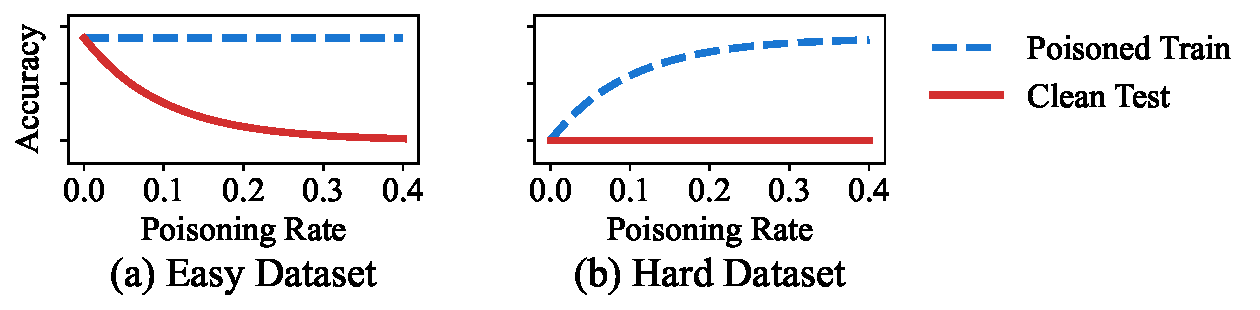
\includegraphics[width=\columnwidth]{images_poisoning/fake_acc.pdf}
    \caption[Theoretical Performance Degradation Under Poisoning Attacks.]{The theoretical performance degradation from poisoning attacks at various rates for easy and hard datasets.}
    \label{fig.fake}
\end{figure}

From a defender's perspective,
Equation~\ref{eq1} can be interpreted as the adversary making the discrepancy between $f$ and $f'$ as large as possible.
Since the training process optimizes $\ell(\Dpo, f')$ on poisoned data,
we know $\ell(\Dpo, f')$ must be significantly smaller than $\ell(\Dpo, f)$.
Because loss is directly linked to the model's accuracy, poisoning attacks can be detected by comparing the clean and the poisoned accuracy.

\subsection{Fast Adversarial Label-Flipping Attack}
\label{sec:method:falfa}

n this section, we introduce a novel label poisoning attack, \falfa (\emph{Fast Adversarial Label Flipping Attack}).
We directly align \falfa with the adversary's goal, making it an extremely effective untargeted attack.
This attack demonstrates that even with the lowest capability (only poisoning labels), it can have a significant negative impact on the performance of neural networks (NNs).

\falfa is derived from Equation~\ref{eq1}, the general form of an untargeted poisoning attack.
Label poisoning attacks are a special type of untargeted poisoning attack, where the adversary's capability is limited to only manipulate labels.
In a label poisoning attack, the attacker's capability is restricted to modifying labels.
In a binary classification task, given $\ytr:=\{y_i\}^n_{i=1}$ and the percentage $\epsilon$ of examples  the adversary can modify,
we hope to find the optimal solution of $\ypo:=\{y'_i\}^n_{i=1}$ to maximize the difference between $f$ and $f'$.
We rewrite Equation~\ref{eq1} with the adversary's cost constants as:
\begin{equation}
    % \footnotesize
    \begin{aligned}
        \min_{\ypo} \quad   & \ell(f'(\Xtr), \ypo) - \ell(f(\Xtr), \ypo)           \\
        \textrm{s.t.} \quad & \sum_{i=1}^{n} |y'_i - y_i| \leq n \epsilon,         \\
        \quad               & y'_i \in \{0, 1\}  \; \text{for } i = 1,  \ldots, n.
    \end{aligned}
    \label{eq2}
\end{equation}
Let us consider a NN classifier, the outputs are normalized by the Softmax function:
\begin{equation}
    % \footnotesize
    p_i = \text{Softmax}(x_i) = \frac{\exp{x_i}}{\sum_j\exp{x_j}}
\end{equation}
and it is optimizing the \emph{Cross Entropy Loss}:
\begin{equation}
    % \footnotesize
    \ell(p_i, y_i) = y_i[-\log(p_i) + \log(1-p_i)]
\end{equation}
By expanding the objective function in Equation~\ref{eq2}, we have the following:
\begin{equation*}
    % \footnotesize
    \begin{aligned}
          & \ell(f'(\Xtr), \ypo) - \ell(f(\Xtr), \ypo)                  \\
        = & \ypo[(-\log(p') + \log(1-p'))] - \ypo[-\log(p) + \log(1-p)] \\
        = & \ypo[(-\log(p') + \log(1-p')) - (-\log(p) + \log(1-p))]     \\
        = & (\alpha - \beta)\ypo
    \end{aligned}
    \label{eq3}
\end{equation*}

\noindent with $\alpha := -\log(p') + \log(1-p')$ and $\beta := -\log(p) + \log(1-p)$.
Then, Equation~\ref{eq2} becomes a linear programming problem with non-linear constraints.
Additionally, the $\beta$ term only depends on the original classifier $f$ and clean data $\Dtr$, so it is a constant and can be computed beforehand.

If Equation~\ref{eq2} were linear, it would be simple to solve, but its inequality constraint contains the absolute operation rendering it nonlinear.
We can remove this operator by considering all permutations \cite{paudice2018label},
but this approach is computationally expensive.
However, since the problem is a binary classification, we can simplify it using a multiplier
$\lambda$ with $\lambda = 1 \text{ if } y_i = 0$ and $-1$ otherwise.
Thus, $|y'_i-y_i|$ and $\lambda \cdot (y_i' - y_i)$ are equivalent, because if $y'_i=y_i$,
$\lambda$ is irrelevant.
Since $\lambda$ only depends on $\ytr$, it is a constant vector.
This transformation significantly reduces the computation cost.

We can further simplify Equation~\ref{eq2} by relaxing the boundary condition.
If we use the {\em Simplex} method to solve this linear programming problem, we can replace $y'_i \in \{0, 1\}$ by $0 \leq y'_i \leq 1$, because the solution is guaranteed on the edges.
Therefore, Equation~\ref{eq2} becomes a linear programming problem:
\begin{equation}
    % \footnotesize
    \begin{aligned}
        \min_{\ypo} \quad   & (\alpha - \beta)\ypo                                      \\
        \textrm{s.t.} \quad & \lambda \cdot \ypo \leq  n \epsilon + \lambda \cdot \ytr, \\
        \quad               & 0 \leq y'_i \leq 1  \; \text{for } i = 1,  \ldots, n.
    \end{aligned}
    \label{eq4}
\end{equation}

\begin{algorithm}[t!]
    \footnotesize
    \caption{Fast Adversarial Label Flipping Attack (\falfa)}
    \begin{algorithmic}[1]
        \Require
        Original training set $\Dtr:=\{(\Xtr, \ytr)\}$, budget parameter $\epsilon$, classifier $f$ trained on $\Dtr$
        \Ensure
        Poisoned training labels $\ypo$
        \State $p \gets \text{Softmax}(f(\Xtr))$;
        \State $\beta \gets -\log(p) + \log(1-p)$;
        \State $\lambda \gets 1 \text{ if } (y_i == 1) \text{ else } -1,  \forall y_i \in \ytr$;
        \State $\ypo \gets \text{Randomly flip } n \cdot \epsilon \text{ examples on } \ytr$;
        \State $f' \gets f$;
        \While{$\ypo$ does not converge}
        \State Retrain classifier $f'$ using $(\Xtr, \ypo)$;
        \State $p' \gets \text{Softmax}(f'(\Xtr))$;
        \State $\alpha \gets - \log(p') + \log(1-p')$;
        \State Update $\ypo$ by solving Eq.~\ref{eq4};
        \EndWhile
        \State \textbf{return} $\ypo$;
    \end{algorithmic}
    \label{alg.flfa}
\end{algorithm}

The full algorithm of \falfa is shown in Algorithm~\ref{alg.flfa}.
\falfa has the following advantages compared with existing label poisoning attacks that we have covered in Section~\ref{sec:survey:poison_attacks}:
\begin{enumerate}
    \item It is efficient on NN models. Apart from the poisoned classifier $f'$ itself, only $p'$ and $\alpha$ require updates. Anything else is constant and can be computed beforehand.
    \item It is invariant to poisoning rates. Equation~\ref{eq4} can be solved by a linear programming solver. Thus, we update $\ypo$ without looping through all permutations.
    \item It is guaranteed solvable at any poisoning rate. We randomly flip $n \cdot \epsilon$ examples on $\ytr$ and use it as the {\em initial solution} for $\ypo$. Since the initial solution is always feasible, Equation~\ref{eq4} is guaranteed to have a feasible solution.
\end{enumerate}
Noting that \falfa is not limited to NNs, it applies to any classifier that uses a \emph{Cross Entropy Loss} function.

\section{Experiments}
\label{sec:exp}

\subsection{Experimental Setup}

\subsubsection{Datasets}
% SUMMARY: Real datasets
We evaluate \diva on 10 real-world datasets from the UCI ML repository \cite{Dua2019}.
We apply standardization on all datasets during the preprocessing.

For datasets that are multi-class classification tasks, we convert the dataset into binary based on the following:
\begin{itemize}
    \item \textbf{Abalone:} If the `Rings' attribute is less than 10, we assign the example to the negative class,  else we assign to the positive class. We exclude the categorical attribute, `Sex', and the output label, `Rings', from the inputs.

    \item \textbf{CMC:} has 3 output classes:
          \begin{enumerate*}
              \item No-use,
              \item Long-term, and
              \item Short-term
          \end{enumerate*}.
          If the class is `No-use', we assign it to the negative class, else we assign it to the positive class.

    \item \textbf{Texture:} has 10 output classes. We use a subset which contains examples labeled as `3' and `9'.
          If the class is `3', assign it to the negative class, else assign it to the positive class.

    \item \textbf{Yeast:} has 10 output classes. We select `0' and `7', the top two classes sorted by sample size.
          If the class is `0', assign it to the negative class, else assign to the positive class.
\end{itemize}
All datasets use an 80-20 training and test split.
We use {\em leave-one-dataset-out} cross-validation to evaluate the performance of \diva by training the meta-learner on 9 datasets and evaluating on the remaining one.

\subsubsection{Classifiers' Performance}

We include \falfa, ALFA \cite{xiao2012adversarial} and Poisoning SVM (PoisSVM) \cite{biggio2012poisoning}.
For \falfa, we train a NN model with 2 hidden layers (128 neurons each) using Stochastic Gradient Descent for a maximum of 400 epochs, learning rate $0.01$, and mini-batch size 128.
The baseline performance of these classifiers trained on clean data are shown in Table~\ref{tab.datasets}.

% TABLE: Summary of datasets.
\begin{table}[ht!]
    \footnotesize
    \centering
    \caption[Summary of Real-World Data]{Summary of the training set size ($n$), number of features ($m$), Positive Label Rate (PLR), average accuracy (\%) for training and test sets across all classifiers, and difficulty (\underline{E}asy/\underline{N}ormal/\underline{H}ard).
    }
    \begin{tabular}{@{\hskip2pt}l@{\hskip2pt}|@{\hskip2pt}r@{\hskip2pt}|@{\hskip2pt}r@{\hskip2pt}|@{\hskip2pt}r@{\hskip2pt}|@{\hskip2pt}r@{\hskip2pt}|@{\hskip2pt}r@{\hskip2pt}|@{\hskip1pt}c@{\hskip1pt}}
        \toprule
        Dataset      & $n$  & $m$ & PLR  & Train Acc.    & Test Acc.     & Diff. \\
        \midrule
        Abalone      & 1600 & 7   & 0.50 & $79.9\pm0.7$  & $76.5\pm0.5$  & N     \\
        Australian   & 552  & 14  & 0.45 & $91.5\pm3.1$  & $81.9\pm2.1$  & N     \\
        Banknote     & 1097 & 4   & 0.44 & $100.0\pm0.0$ & $100.0\pm0.0$ & E     \\
        Breastcancer & 455  & 30  & 0.63 & $99.3\pm0.2$  & $95.0\pm2.5$  & E     \\
        CMC          & 1178 & 9   & 0.77 & $79.9\pm2.8$  & $77.5\pm0.6$  & N     \\
        HTRU2        & 1600 & 8   & 0.50 & $94.8\pm0.5$  & $92.6\pm0.9$  & E     \\
        Phoneme      & 1600 & 5   & 0.50 & $89.7\pm6.3$  & $85.6\pm1.3$  & N     \\
        Ringnorm     & 1600 & 20  & 0.50 & $99.4\pm0.4$  & $97.8\pm1.1$  & E     \\
        Texture      & 800  & 40  & 0.50 & $100.0\pm0.0$ & $99.8\pm0.5$  & E     \\
        Yeast        & 713  & 8   & 0.48 & $73.5\pm4.7$  & $65.8\pm1.6$  & H     \\
        \bottomrule
    \end{tabular}
    \label{tab.datasets}
\end{table}

For ALFA and PoisSVM, we use SVM with an RBF kernel and the parameters $C$ and $\gamma$ tuned by a 5-Fold CV.
We also include {\em Stochastic Label Noise} (SLN) as a baseline attack, which randomly flips a percentage of labels.
Moreover, PoisSVM is an {\em insertion attack}, so the poisoning rate is the percentage of additional examples added to the dataset.

\subsection{Experimental Results}

We present the performance loss at a poisoning rate of $10\%$ in Table~\ref{tab.err10}.
This table shows test accuracy differences before and after the attack.
At the poisoning rate of $10\%$, SLN has no meaningful impact on NN models' performance with an average performance loss of $0.98\%$,  demonstrating that NNs are robust against SLN at $10\%$.
\falfa and ALFA are tied in top-ranked attacks with 7 out of 10 datasets on paired two sample T-tests with $\alpha$ set to $0.1$.
\falfa outperforms ALFA by a large margin on the Phoneme and Ringnorm datasets but is bested by ALFA on the Abalone and Yeast datasets.

\begin{table}[ht!]
    \footnotesize
    \centering
    \caption[Performance Loss Under Label Poisoning Attacks]{Performance loss (\%) after attacked by a poisoning attack with 10\% poisoning rate. Top ranked attacks are marked in \textbf{bold}.}
    \begin{tabular}{l|@{\hskip2pt}r@{\hskip2pt}|@{\hskip2pt}r@{\hskip2pt}|@{\hskip2pt}r@{\hskip2pt}|@{\hskip2pt}r@{\hskip2pt}}
        \toprule
        Dataset      & SLN          & PoisSVM               & ALFA                  & \falfa                \\
        \midrule
        Abalone      & $0.8\pm0.7$  & $1.8\pm0.8$           & $\mathbf{9.5\pm1.9}$  & $7.7\pm1.7$           \\
        Australian   & $0.7\pm0.5$  & $4.5\pm3.9$           & $\mathbf{4.9\pm4.0}$  & $\mathbf{8.3\pm3.8}$  \\
        Banknote     & $1.4\pm2.3$  & $1.1\pm1.1$           & $\mathbf{10.9\pm2.5}$ & $\mathbf{10.3\pm2.9}$ \\
        Breastcancer & $2.5\pm0.7$  & $5.3\pm4.6$           & $\mathbf{7.2\pm2.0}$  & $\mathbf{9.1\pm2.7}$  \\
        CMC          & $-0.2\pm0.7$ & $\mathbf{15.1\pm4.7}$ & $3.5\pm3.0$           & $5.7\pm3.3$           \\
        HTRU2        & $0.7\pm0.3$  & $0.7\pm1.3$           & $\mathbf{9.2\pm3.1}$  & $\mathbf{9.4\pm2.4}$  \\
        Phoneme      & $3.5\pm2.9$  & $0.9\pm2.1$           & $6.8\pm0.7$           & $\mathbf{11.6\pm2.1}$ \\
        Ringnorm     & $0.1\pm0.3$  & $1.7\pm0.5$           & $3.2\pm2.5$           & $\mathbf{6.4\pm2.9}$  \\
        Texture      & $0.5\pm1.1$  & $1.2\pm0.8$           & $\mathbf{7.9\pm4.6}$  & $\mathbf{4.9\pm3.9}$  \\
        Yeast        & $-0.2\pm1.6$ & $1.9\pm3.8$           & $\mathbf{10.4\pm4.9}$ & $2.3\pm4.6$           \\
        \bottomrule
    \end{tabular}
    \label{tab.err10}
\end{table}


Figure \ref{fig.real_acc} illustrates the relationship between the poisoned training accuracy and the clean test accuracy when a classifier is poisoned at various rates\footnote{We are only able to run PoisSVM up to 30\% poisoning rate using the implementation provided by the original paper \cite{biggio2012poisoning}.}.
We observe that \falfa and ALFA reliably degrade the classifier performance on all three datasets. However, PoisSVM is substantially weaker.

Previous works use the test classification error as the sole performance metric to benchmark the poisoning attacks \cite{ho2002complexity,koh2022stronger,paudice2018label}.
However, this does not fully reflect the impact of poisoned labels.
To conceal an attack from the user, keeping the training accuracy (dashed lines in Figure \ref{fig.real_acc}) stationary is equally essential.
The behavior of SLN (gray lines in Figure~\ref{fig.real_acc}) is different from other attacks, as the training and test accuracy fall at a similar rate, highlighting the key motivation of this research.

\begin{figure}[ht!]
    \centering
    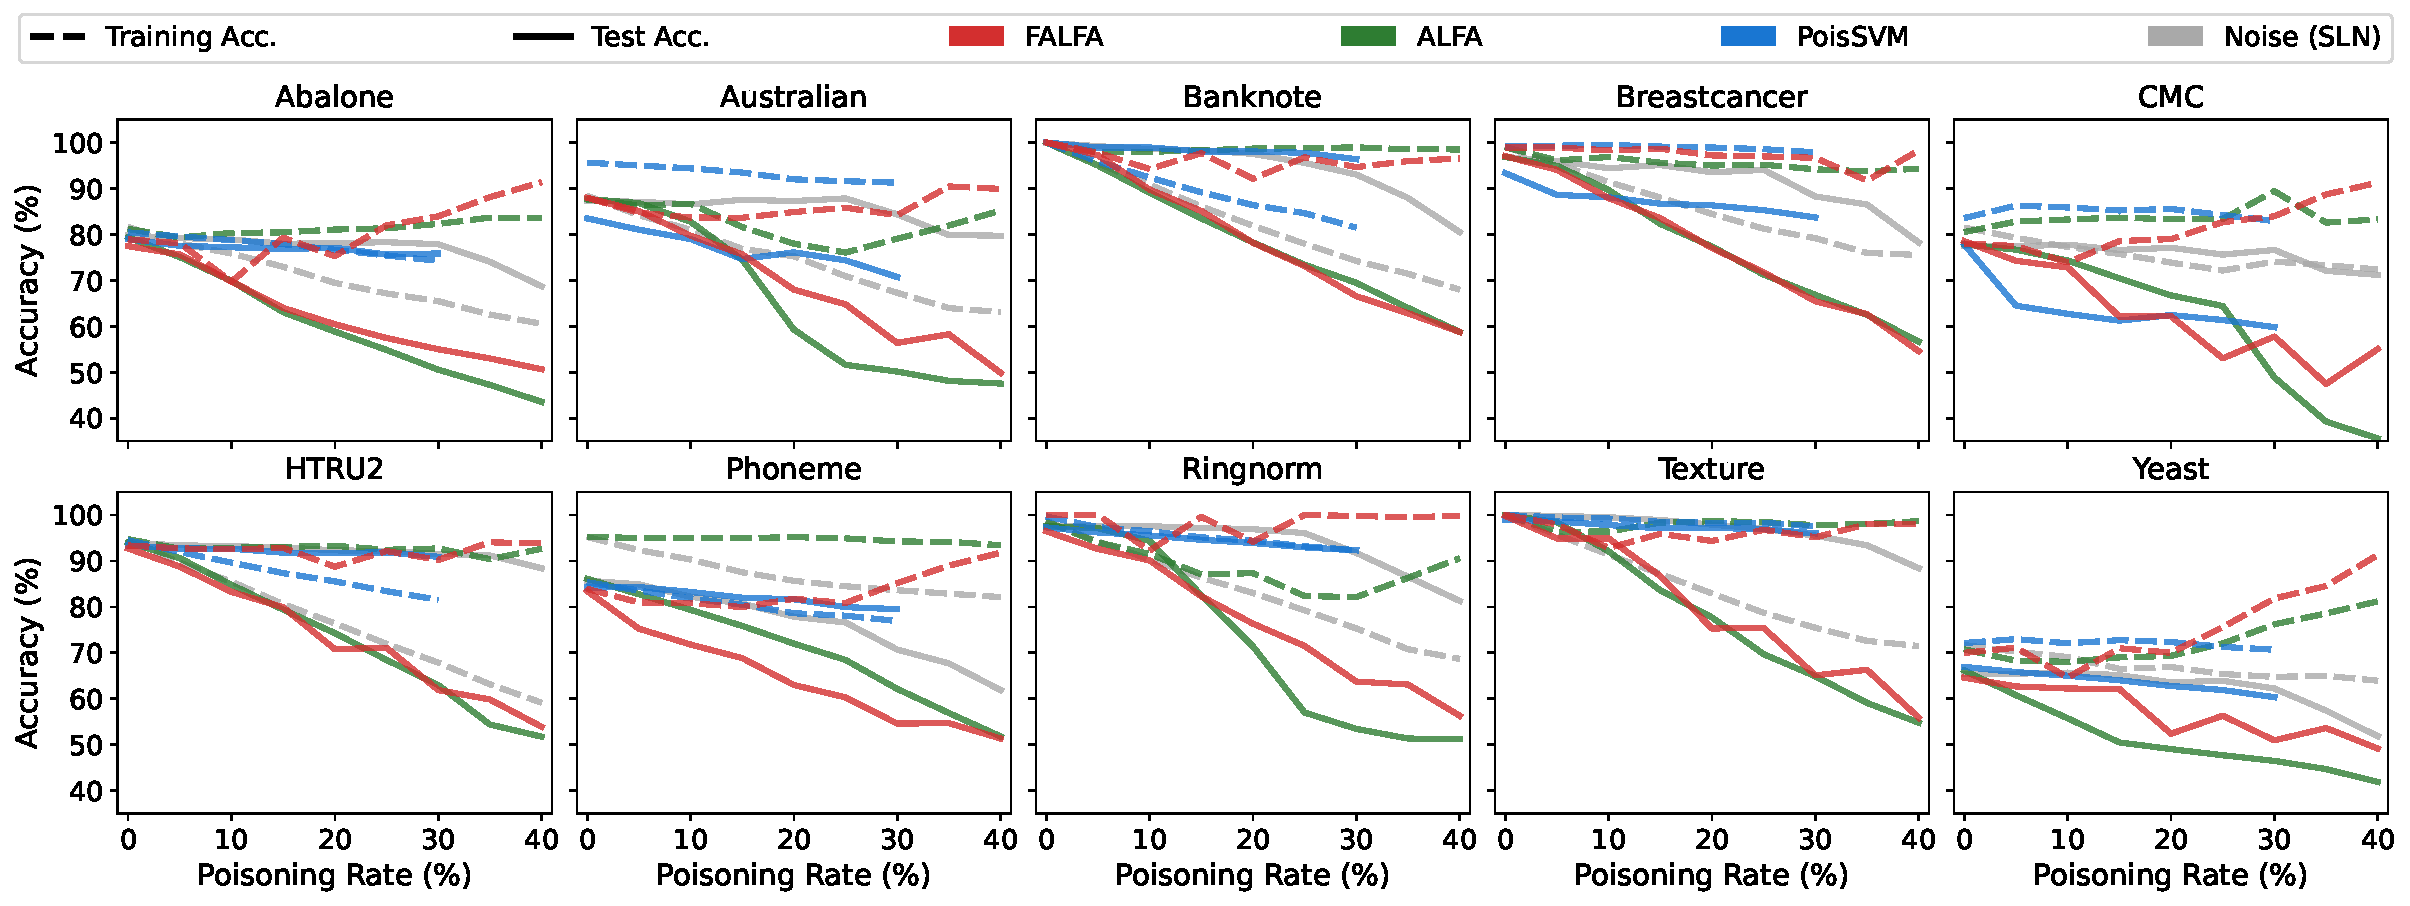
\includegraphics[width=\columnwidth]{images_poisoning/flfa_acc_all.pdf}
    \caption[Training and Test Accuracy Under Poisoning Attacks]{
        The training and test accuracy at various poisoning rates exhibit similar patterns under different attacks on the same dataset. However, the difficulty of the classification task has a large influence on the behavior of attacks.
    }
    \label{fig.real_acc}
\end{figure}

Given a difficult classification task,
an increasing poisoning rate has a limited impact on the testing accuracy, such as the Yeast dataset in Figure~\ref{fig.real_acc}.
Meanwhile, the training accuracy on poisoned data rises.
This pattern is observed in poisoning attacks, but not in noise.
We believe this is due to the poisoning attacks optimizing the second term in Equation~\ref{eq2}.
When the testing accuracy is close to random levels, an attack algorithm can no longer maximize the loss on test data; it will minimize the loss on the training data instead.
Thus, the classifier becomes more likely to overfit the poisoned training set.
\diva takes advantage of this characteristic, since the discrepancy between training and test accuracy still exists, despite the limited room for an increased classification error.
However, weak attacks may fail in this scenario, as seen in PoisSVM leading to only $6.6\%$ performance loss at a $30\%$ poisoning rate on Yeast. \diva would not detect this case, as it will be seen as an unsuccessful attack (see Table \ref{tab:attack-matrix}).


\subsubsection{Time Complexity of \falfa}

\falfa is more computationally efficient than ALFA and PoisSVM by a substantial margin.
Linear programming is an exponential-time algorithm, where the time complexity is around $O(n^{2.5})$.
Xiao {\em et al.}'s ALFA creates a copy of $\ytr$ in the linear programming step, so $n$ is essentially doubled.
Paudice {\em et al.}'s ALFA on NNs is slower than Xiao {\em et al.}'s, since it traverses all combinations of $\ytr$ instead of using linear programming.
\falfa uses linear programming but without doubling $\ytr$, resulting in an approximately $2^{2.5}\approx5.6$ times faster than ALFA on each iteration.
Our test shows that \falfa converges at 2 iterations on average, but ALFA takes more than 5 iterations to converge.
In the worst-case scenario, \falfa poisons the CMC dataset in $22.4\pm8.6$ secs, while ALFA requires $405.8\pm348.4$ secs, and PoisSVM took over 2 hours.
We observe the minimal difference on BreastCancer, where \falfa completes the task at $5.3\pm1.9$ secs, and it takes ALFA $7.4\pm5.6$ secs.


\section{Conclusion and Future Work}
\label{sec:conclusion}

Place holder

%
% ---- Bibliography ----
%
% BibTeX users should specify bibliography style 'splncs04'.
% References will then be sorted and formatted in the correct style.
%
\bibliographystyle{splncs04}
\bibliography{references}
%
\end{document}
